% ta med damping på DP-delle

\documentclass[aspectratio=169,xcolor=dvipsnames]{beamer}
%\usetheme{SimplePlus}

\usepackage{hyperref}
\usepackage{graphicx} % Allows including images
\usepackage{booktabs} % Allows the use of \toprule, \midrule and \bottomrule in tables

%----------------------------------------------------------------------------------------
%	TITLE PAGE
%----------------------------------------------------------------------------------------

\title[PLS]{PLS IO koblinger} % The short title appears at the bottom of every slide, the full title is only on the title page
%\subtitle{Subtitle}

\author[Fred-Olav] {Fred-Olav Mosdal}

\institute[Gand VGS] % Your institution as it will appear on the bottom of every slide, may be shorthand to save space
{
    Gand VGS \\
    VG3 Automasjon }
\date{\today} % Date, can be changed to a custom date


%----------------------------------------------------------------------------------------
%	PRESENTATION SLIDES
%----------------------------------------------------------------------------------------

\begin{document}
\begin{frame}
\titlepage
\end{frame}



\begin{frame}
	\frametitle{Styringssystemers tre deler}
	\begin{columns}
		\begin{column}{0.5\textwidth}
	\begin{itemize}
		\item Inngangsenheter
		\item styreenheter 
		\item utgangsenheter
	\end{itemize}
		\end{column}
		\begin{column}{0.5\textwidth}
	$$\includegraphics[width=1\textwidth]{../output/noGPLimages/pls01.png}$$
		\end{column}
	\end{columns}
\end{frame}


\begin{frame}
	\frametitle{PLS-ens opprinnelse}
	\begin{columns}
		\begin{column}{0.5\textwidth}
			Ble lansert som erstatning for relestyringer\\
			Opprinnelsen sees fremdeles i det mest vanlige programeringsspråket for PLS-er Ladder Logic Diagram
		\end{column}
		\begin{column}{0.5\textwidth}
	$$\includegraphics[width=1\textwidth]{../output/noGPLimages/Modicon 084.jpg}$$
			\url{https://www.engineering.com/programmable-logic-controllers-the-evolution-of-a-disruptive-technology/}
		\end{column}
	\end{columns}
\end{frame}


\begin{frame}
	\frametitle{Eksempler på PLS-er}
$$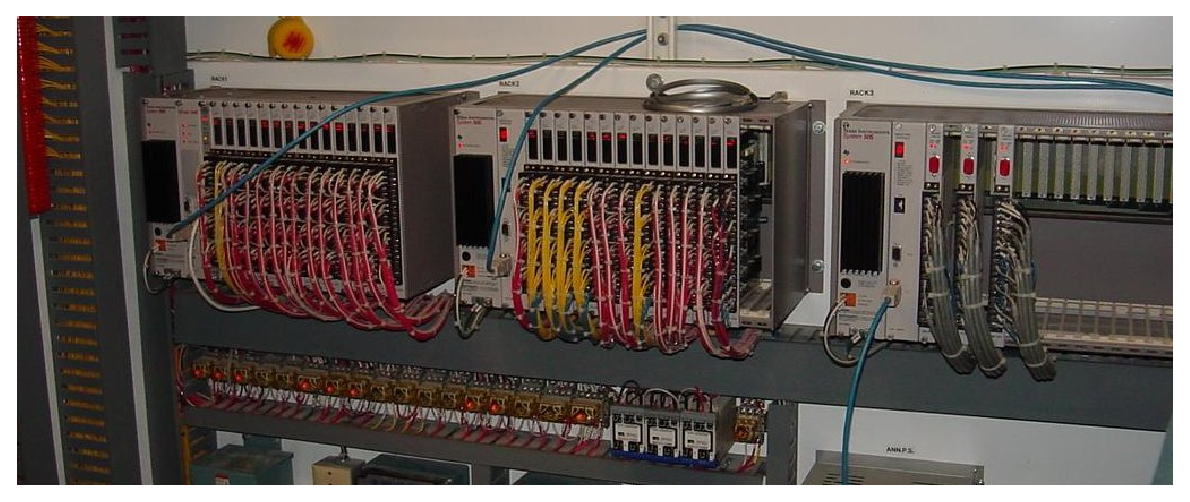
\includegraphics[width=1\textwidth]{plc_001.eps}$$
\end{frame}

\begin{frame}
	\frametitle{Eksempler på PLS-er}
$$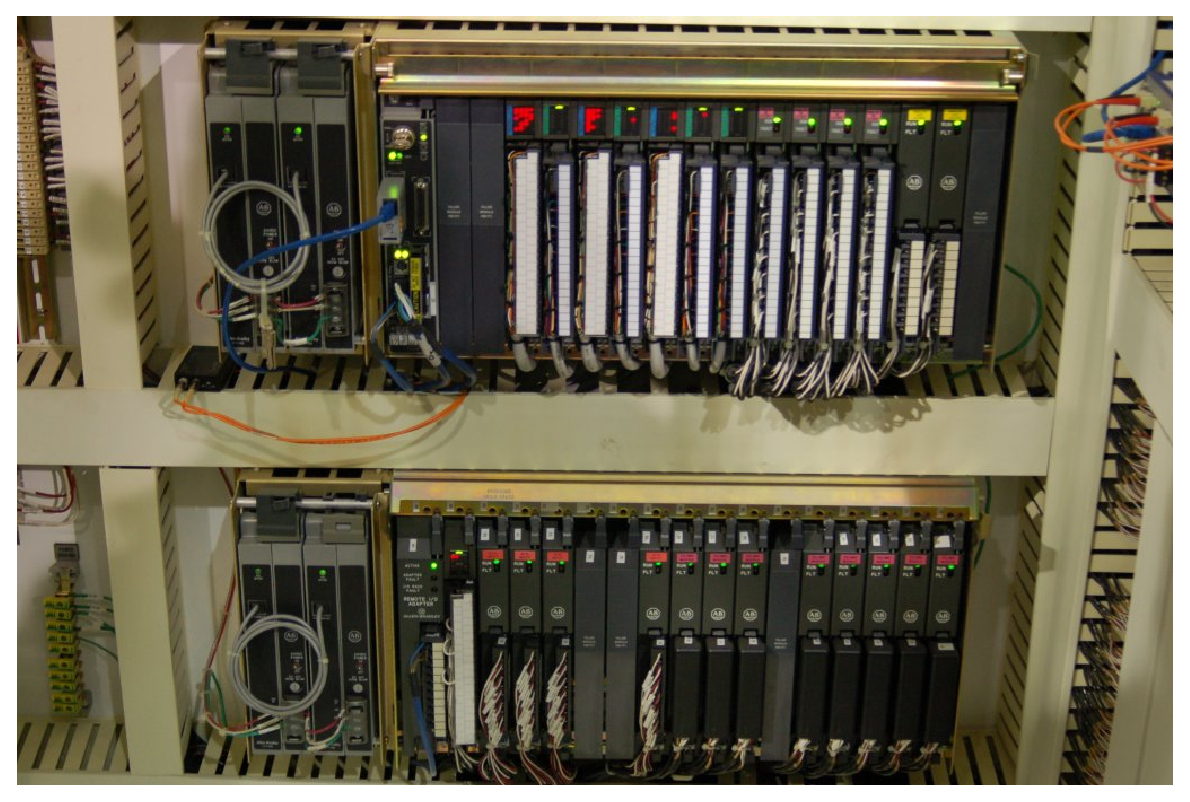
\includegraphics[width=0.8\textwidth]{plc_002.eps}$$
\end{frame}

\begin{frame}
	\frametitle{Eksempler på PLS-er}
$$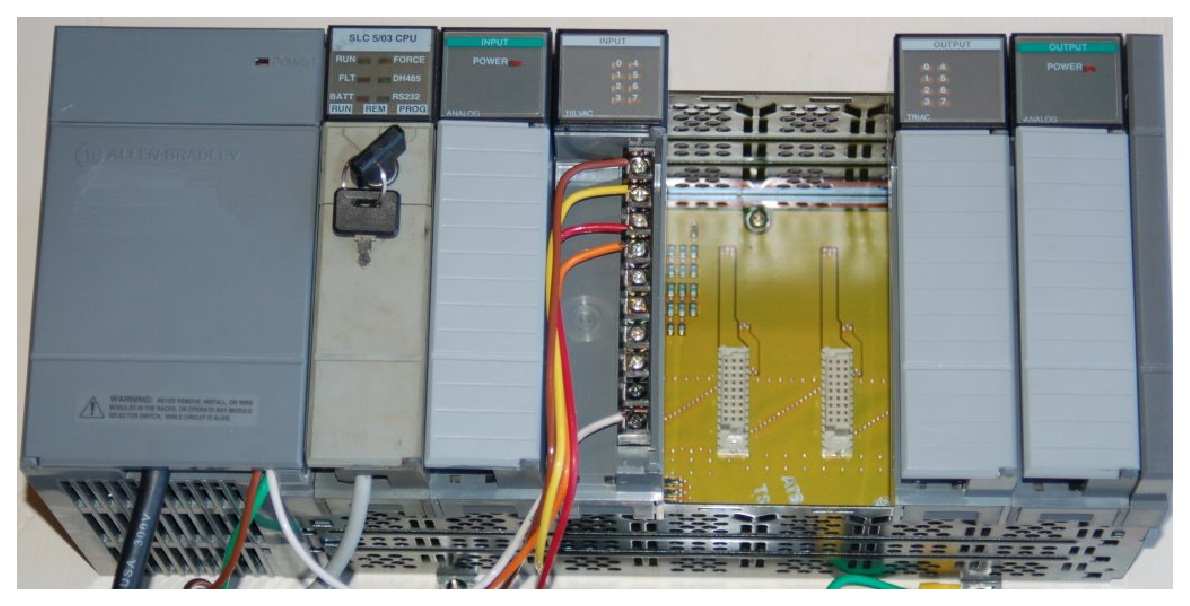
\includegraphics[width=0.9\textwidth]{plc_017.eps}$$
\end{frame}
\begin{frame}
	\frametitle{Eksempler på PLS-er}
$$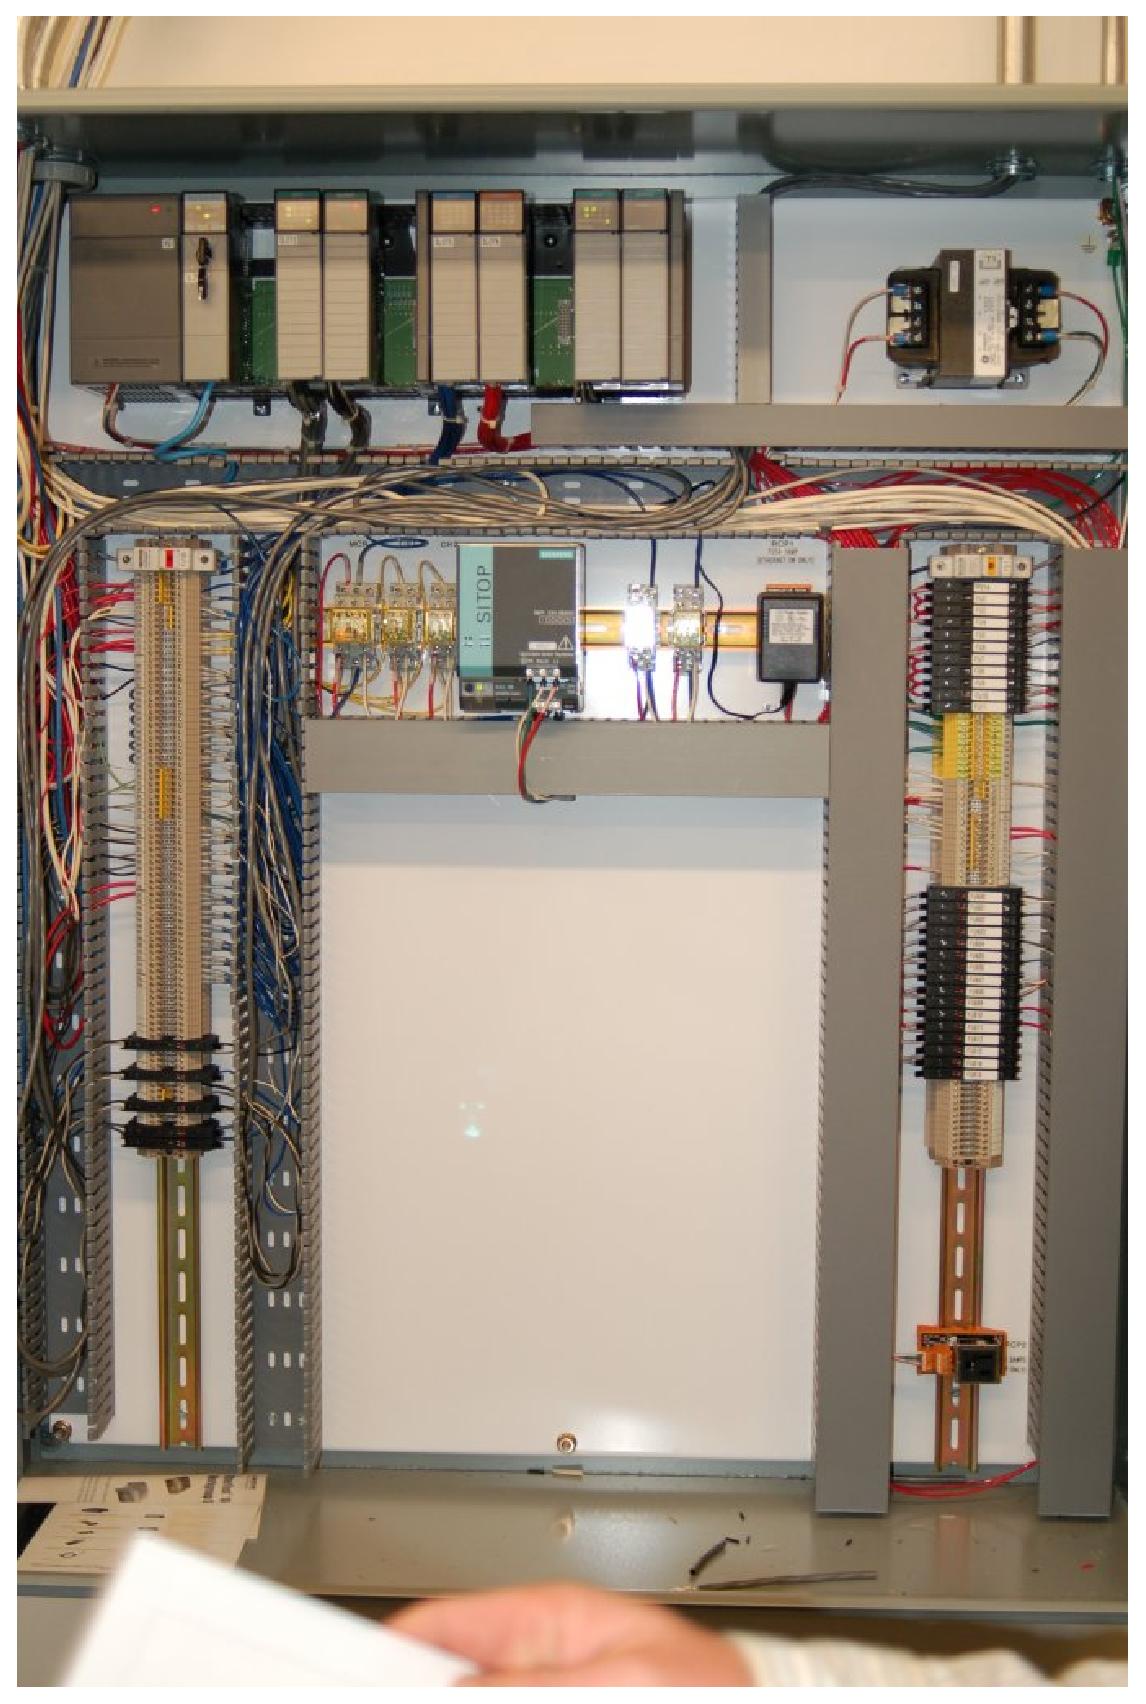
\includegraphics[width=0.8\textwidth]{plc_018.eps}$$
\end{frame}
\begin{frame}
	\frametitle{Eksempler på PLS-er}
$$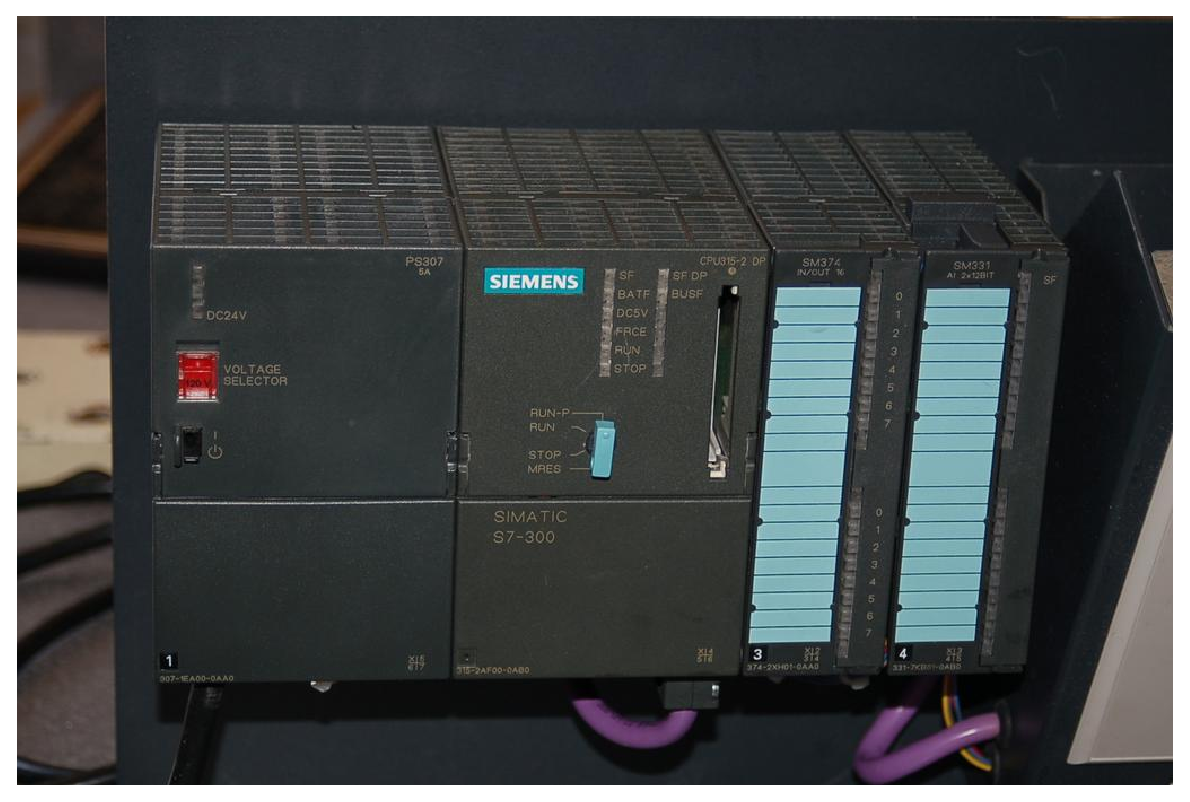
\includegraphics[width=0.7\textwidth]{plc_003.eps}$$
\end{frame}
\begin{frame}
	\frametitle{Eksempler på PLS-er}
$$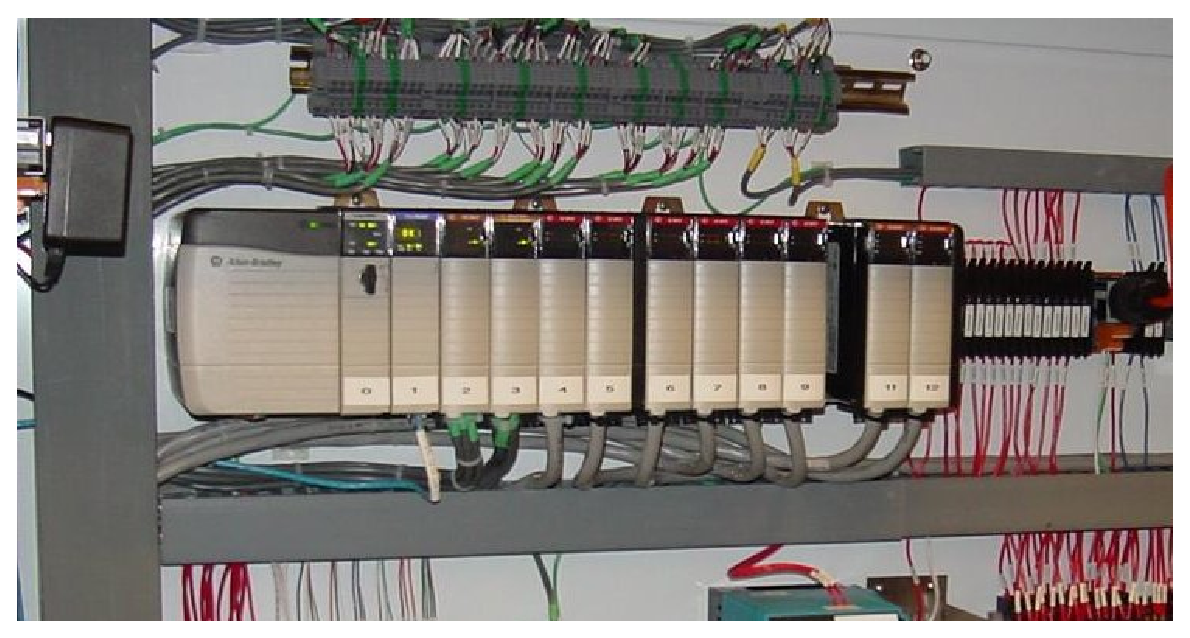
\includegraphics[width=0.9\textwidth]{plc_004.eps}$$
\end{frame}
\begin{frame}
	\frametitle{Eksempler på PLS-er}
$$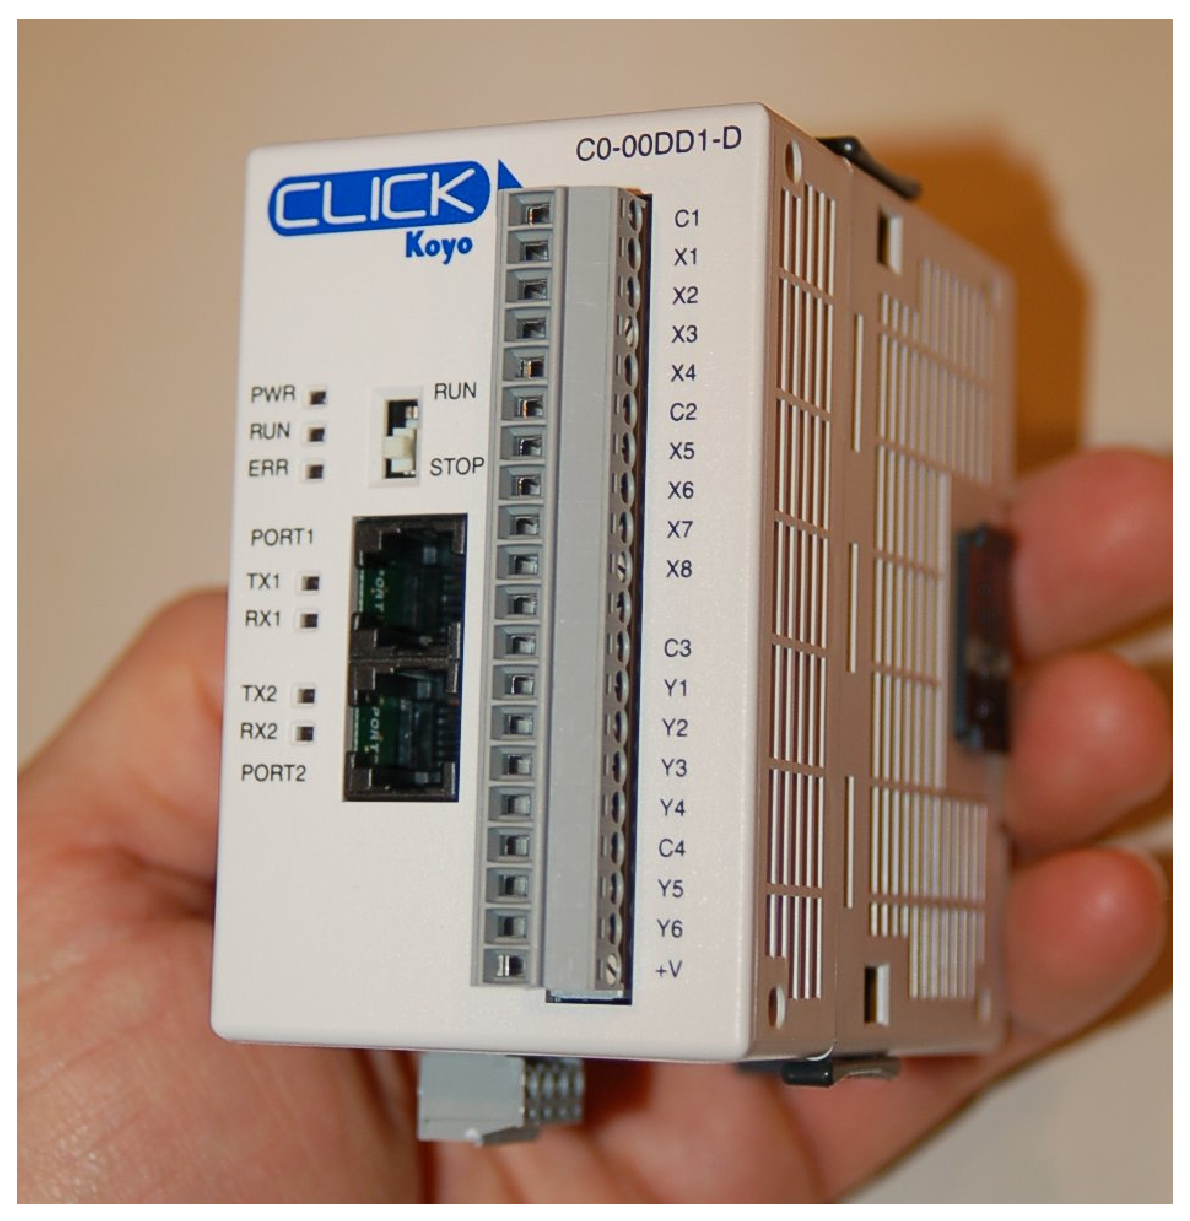
\includegraphics[width=0.5\textwidth]{plc_005.eps}$$
\end{frame}
\begin{frame}
	\frametitle{Eksempler på PLS-er}
$$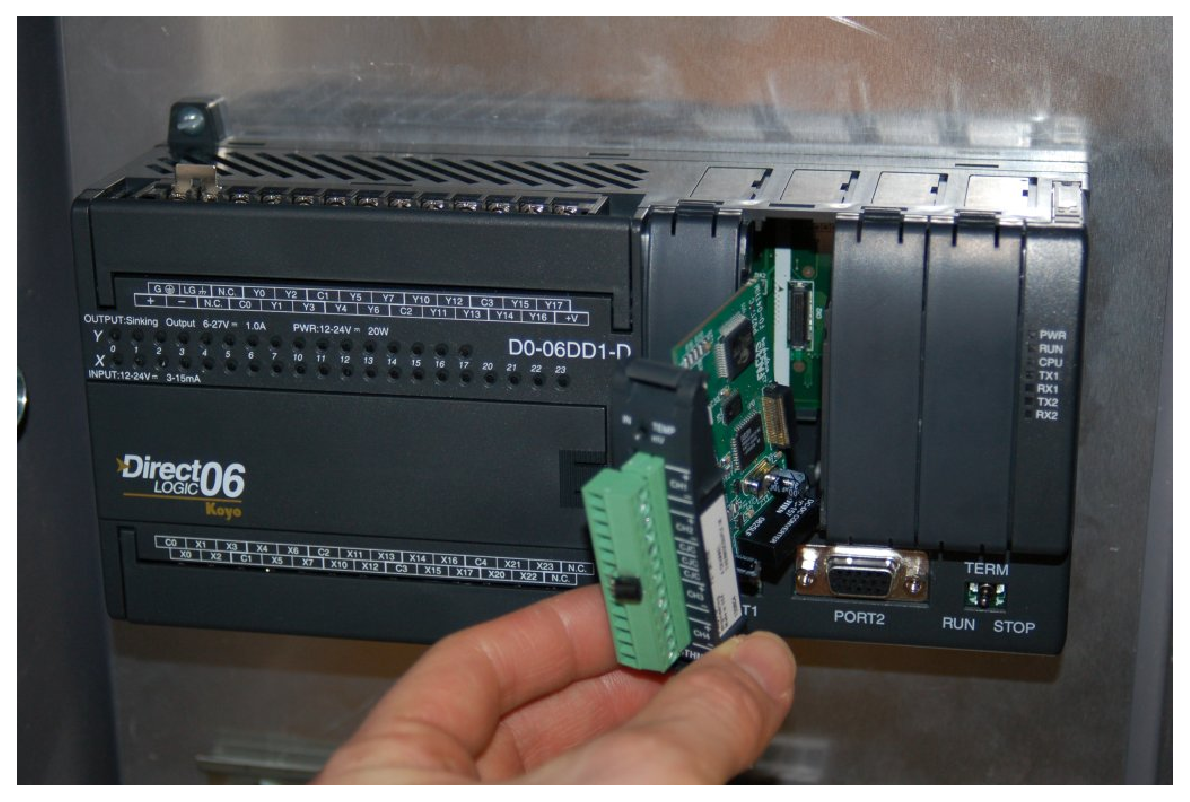
\includegraphics[width=0.8\textwidth]{plc_007.eps}$$
\end{frame}
\begin{frame}
	\frametitle{Eksempler på PLS-er}
$$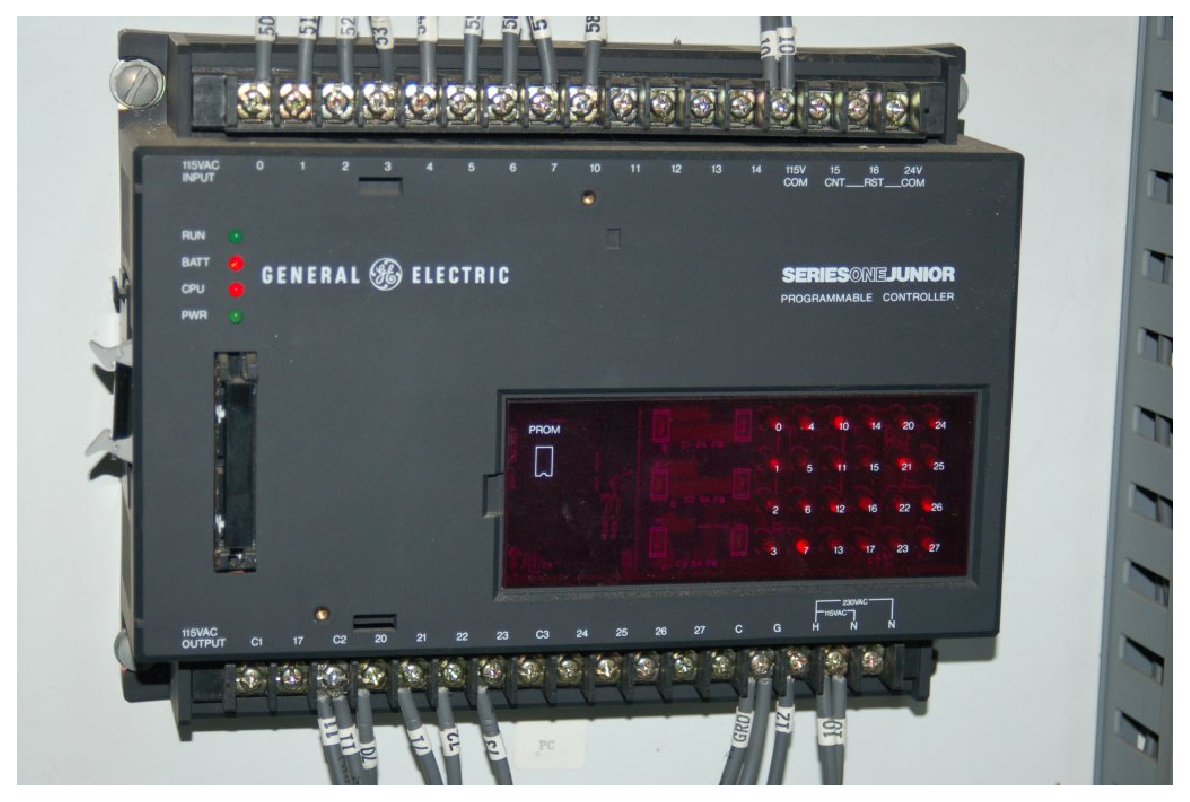
\includegraphics[width=0.8\textwidth]{plc_006.eps}$$
\end{frame}
\begin{frame}
	\frametitle{Inngangs- og utgangs tilkoblinger (IO-er)  }
	\framesubtitle{Tilgang til den virkelige verden}			
$$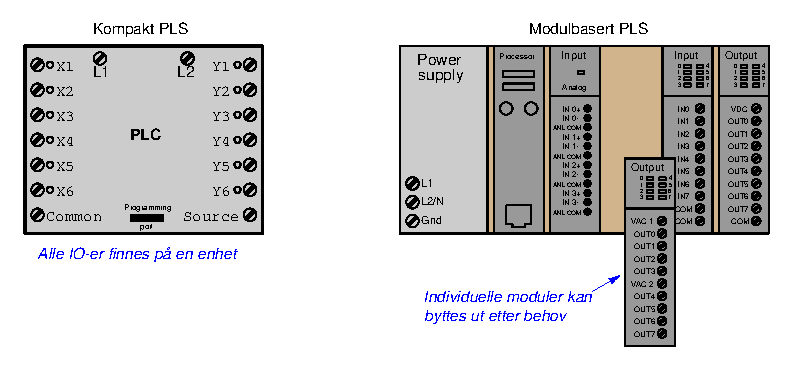
\includegraphics[width=0.8\textwidth]{plc_075.eps}$$
\end{frame}
\begin{frame}
	\frametitle{Inngangs- og utgangs tilkoblinger (IO-er)  }
	\framesubtitle{Tilgang til den virkelige verden}			
$$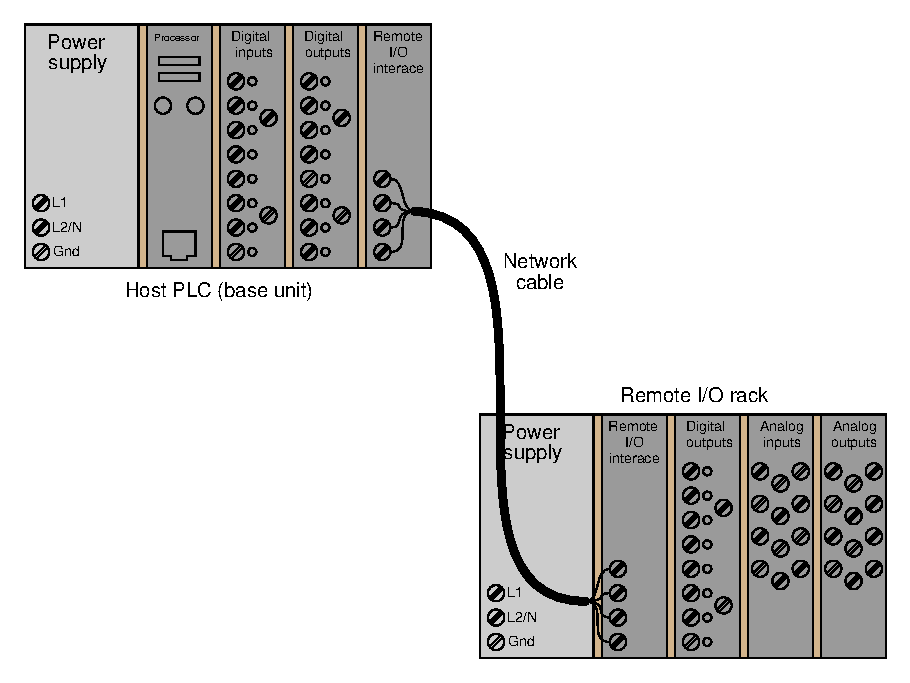
\includegraphics[width=0.6\textwidth]{plc_008.eps}$$
\end{frame}

\begin{frame}
	\frametitle{Digitale IO-er}
	\framesubtitle{Digital inngang}			
	Krav til PLS-IO er satt i \href{https://lese.standard.no/product/2503568/nb}{\textbf{NEK 61131-2}} --
	Eksempel på \href{https://www.ti.com/lit/ab/slla370d/slla370d.pdf}{\textbf{nyere inngang}}
$$\includegraphics[width=0.9\textwidth]{plc_073.eps}$$
\end{frame}

\begin{frame}
	\frametitle{Digitale IO-er}
	\framesubtitle{Digital utgang}			
$$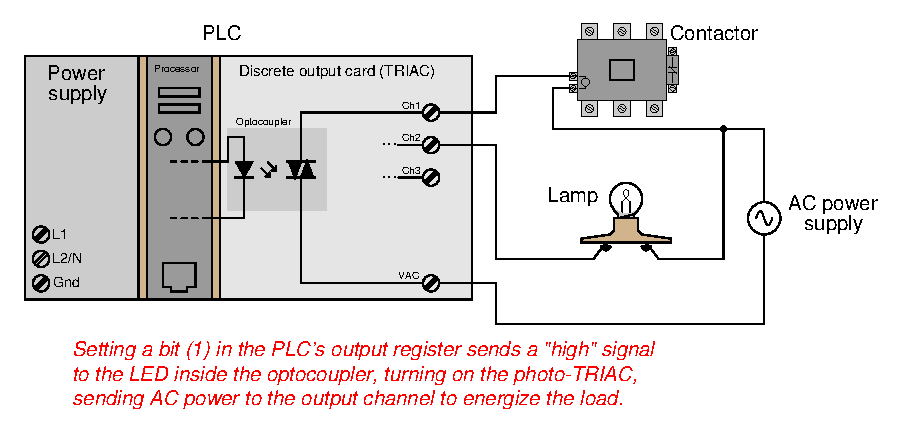
\includegraphics[width=0.9\textwidth]{plc_074.eps}$$
\end{frame}
\begin{frame}
	\frametitle{Sinking og Sourcing}
	\begin{columns}
		\begin{column}{0.5\textwidth}
		\begin{itemize}
			\item Inn- eller utgang som er sinking tar imot strøm 
			\item Inn- eller utgang som er soursing gir ut strøm 
		\end{itemize}	
		\end{column}
		\begin{column}{0.5\textwidth}

$$\includegraphics[width=0.9\textwidth]{plc_009.eps}$$
		\end{column}
	\end{columns}
\end{frame}


\begin{frame}
	\frametitle{Sinking og Sourcing}
	\begin{columns}
		\begin{column}{0.5\textwidth}
			
$$\includegraphics[width=0.9\textwidth]{plc_010.eps}$$
		\end{column}
		\begin{column}{0.5\textwidth}

$$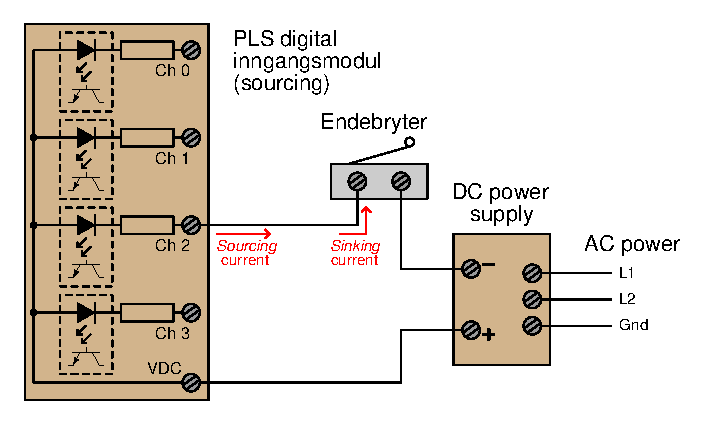
\includegraphics[width=0.9\textwidth]{plc_011.eps}$$
		\end{column}
	\end{columns}
\end{frame}
\begin{frame}
	\frametitle{Sinking og Sourcing}
	\begin{columns}
		\begin{column}{0.5\textwidth}
			
$$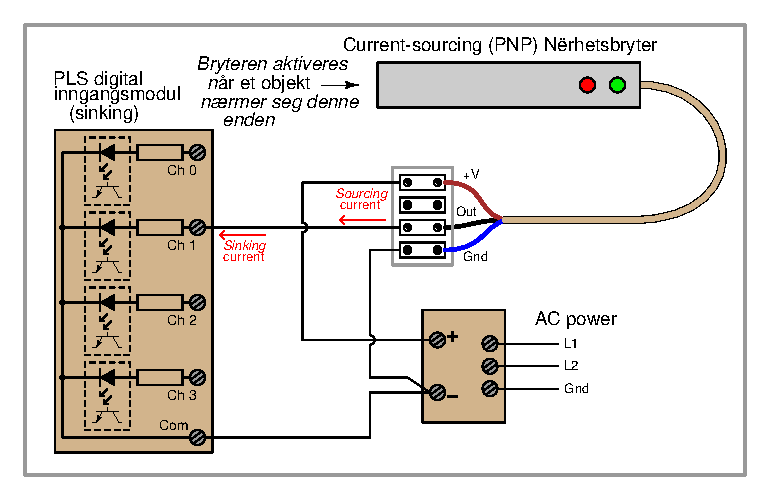
\includegraphics[width=1\textwidth]{plc_012_1.eps}$$
		\end{column}
		\begin{column}{0.5\textwidth}

$$\includegraphics[width=1\textwidth]{plc_012_2.eps}$$
		\end{column}
	\end{columns}
\end{frame}

\begin{frame}{Oppgave}
$$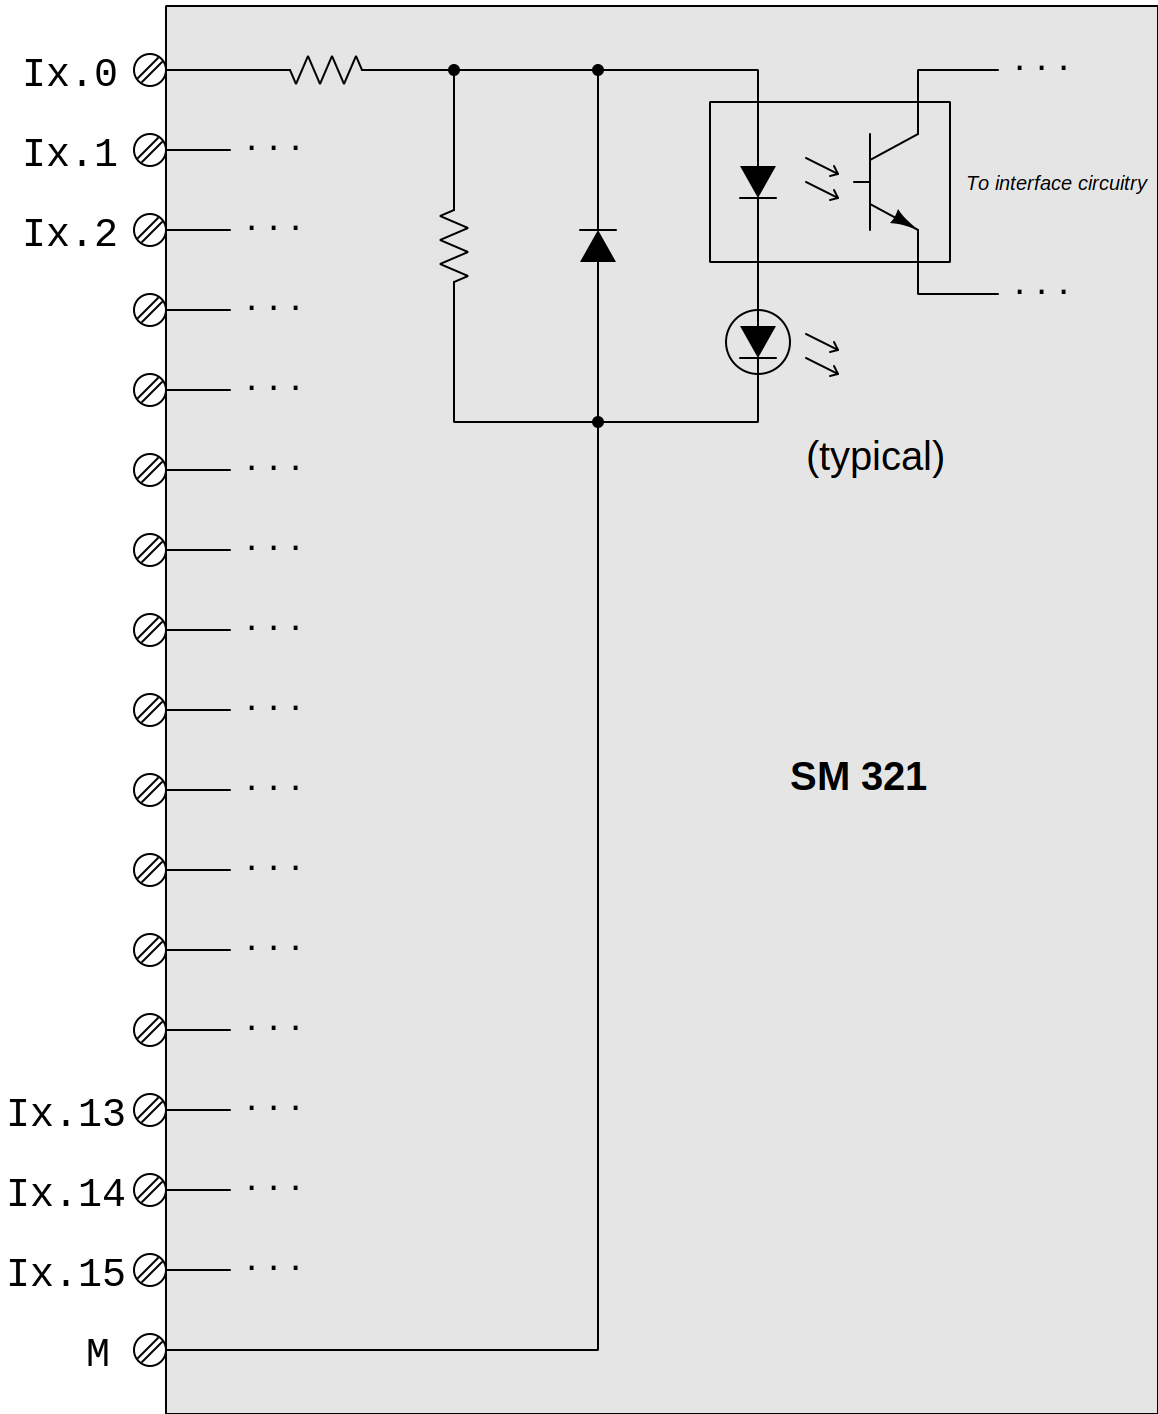
\includegraphics[width=15.5cm]{../src/i04536x01.eps}$$
\end{frame}

\begin{frame}
	\frametitle{Analoge IO-er}
	Hvilke typer analoge IO-er har Wago\\
	sjekk \url{www.wago.no}
\end{frame}

\begin{frame}
	\frametitle{DO med rele}
	\begin{columns}
		\begin{column}{0.5\textwidth}
			Rele utganger :
			\begin{itemize}
				\item kan være potensialfrie
				\item Kan bryte forholdsvis store strømmer (6-10A)
				\item Kan brukes på AC og DC
			\end{itemize}

			
		\end{column}

		\begin{column}{0.5\textwidth}
	$$\includegraphics[width=1\textwidth]{../output/noGPLimages/pls03.png}$$
		\end{column}
	\end{columns}
\end{frame}

\begin{frame}
	\frametitle{DO med transistor (Transistorutgang}
	\begin{columns}
		\begin{column}{0.5\textwidth}
			Transistorutganger:
			\begin{itemize}
				\item bryter mindre strømmer (0.5 og 1 A er vanlig)
				\item bryter raskere en rele utganger
				\item Finnes i NPN eller PNP utgaver
				\item NPN kalles også low side switching
				\item PNP kalles også high side switching
				\item Kan brukes på DC
			\end{itemize}

			
		\end{column}

		\begin{column}{0.5\textwidth}
	$$\includegraphics[width=1\textwidth]{../output/noGPLimages/pls04.png}$$
		\end{column}
	\end{columns}
\end{frame}

\begin{frame}
	\frametitle{DO med triac}
	\begin{columns}
		\begin{column}{0.5\textwidth}
			\begin{itemize}
				\item Kan bryte mindre AC strømmer en releer
				\item Tåler flere bryte sykluser
			\end{itemize}

			
		\end{column}

		\begin{column}{0.5\textwidth}
	$$\includegraphics[width=0.8\textwidth]{../output/noGPLimages/pls05.png}$$
		\end{column}
	\end{columns}
\end{frame}

\begin{frame}
	\frametitle{Galvaniske skiller}
	\begin{columns}
		\begin{column}{0.5\textwidth}
			\begin{itemize}
				\item Isolerer PLS fra spenninger i felt. 
			\end{itemize}

			
		\end{column}

		\begin{column}{0.5\textwidth}
	$$\includegraphics[width=1\textwidth]{../output/noGPLimages/pls06.png}$$
		\end{column}
	\end{columns}
\end{frame}


\begin{frame}
	\frametitle{Analoge IO-er}
	\begin{columns}
		\begin{column}{0.5\textwidth}
			Analoge innganger (AI)
			\begin{itemize}
				\item 1-5 V
				\item 0-10 V
				\item 2-10 V
				\item 4-20 mA
				\item 0-20 mA
				\item RTD ($\Omega$)
				\item termoelement mV
			\end{itemize}

			
		\end{column}

		\begin{column}{0.5\textwidth}
			\href{https://www.contec.com/support/basic-knowledge/daq-control/analog-io/}{link}
			%	$$\includegraphics[width=1\textwidth]{../output/noGPLimages/pls06.png}$$
		\end{column}
	\end{columns}
\end{frame}

\end{document}
